% begin module limit-at-infinity-def
\begin{frame}[t]
\begin{definition}[Limit at Infinity]
Let $f$ be a function defined on some interval $(a,\infty )$.  Then
\[
\lim_{x\rightarrow\infty} f(x) = L
\]
means that the values of $f$ can be made arbitrarily close to $L$ by taking $x$ sufficiently large.
\end{definition}
\uncover<2->{%
\begin{columns}[c]
\column{.3\textwidth}

\psset{xunit=0.4cm, yunit=0.4cm}
\begin{pspicture}(-1, -1)(5,5) 
\psframe*[linecolor=white](-1,-1)(5,4) 
\psaxes[ticks=none, labels=none]{<->}(0,0)(-1,-1)(7,4.5)
%Function formula: (2 (x)+5)/(2 (x)+2) 
\psplot[linecolor=red, plotpoints=1000]{-0.5}{7}{5 x 2 mul add 2 x 2 mul add div }
\psline[linecolor=blue, linestyle=dashed](-1, 1)(7, 1)
\rput[tr](-0.5, 0.8){\tiny $y=L$}
\rput[bl](1.5, 2){\tiny $y=f(x)$}
\end{pspicture} 
%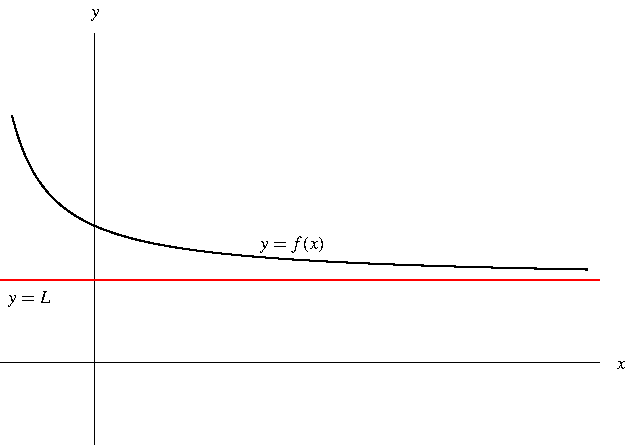
\includegraphics[width=4cm]{curve-sketching/pictures/04-04-asymptotesa.pdf} 
\column{.3\textwidth}
\psset{xunit=0.15cm, yunit=0.15cm}
\begin{pspicture}(-5, -5)(5,5) 
\psframe*[linecolor=white](-5,-5)(5,5) 
\psaxes[ticks=none, labels=none]{<->}(0,0)(-2,-2)(20,12)
%Function formula:3+ (2 (x)+5)/(2 (x)+2)+(20)/(3 (x)+10) (\sin{}(x)) 
\psplot[linecolor=red, plotpoints=3000]{-0.8}{20}{x 57.29578 mul sin 20 10 x 3 mul add div mul 5 x 2 mul add 2 x 2 mul add div add  3 add}
\psline[linecolor=blue, linestyle=dashed](-2, 4)(20, 4)
\rput[tr](-0.5, 3.8){\tiny $y=L$}
\rput[bl](5, 6){\tiny $y=f(x)$}
\end{pspicture} 
%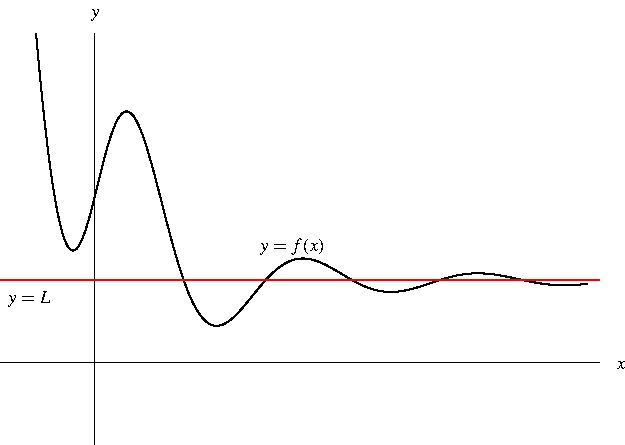
\includegraphics[width=4cm]{curve-sketching/pictures/04-04-asymptotesb.pdf}%
\column{.3\textwidth}
\psset{xunit=0.35cm, yunit=0.35cm}
\begin{pspicture}(-5, -5)(5,5) 
\psframe*[linecolor=white](-5,-5)(5,5) 
\psaxes[ticks=none, labels=none]{<->}(0,0)(-1.5,-1)(8,5)
%Function formula:1+ (x+(x)^{2}+1)/(6+5 (x)+(x)^{2}) 
\psplot[linecolor=red, plotpoints=1000]{-1.5}{8.5}{1 x 2 exp add x add x 2 exp x 5 mul add 6 add div 1 add}
\psline[linecolor=blue, linestyle=dashed](-1, 2)(8.5, 2)
\rput[bl](0.5, 2.2){\tiny $y=L$}
\rput[bl](5, 0.5){\tiny $y=f(x)$}
\end{pspicture} 
%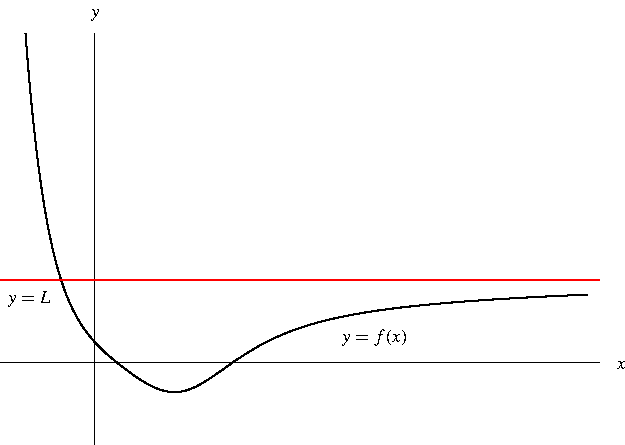
\includegraphics[width=4cm]{curve-sketching/pictures/04-04-asymptotesc.pdf}%
\end{columns}
}%
\begin{itemize}
\item<2->  There are many ways that this can happen.
\item<3->  Other notation: $f(x)\to L$ as $x\to \infty$.
\item<4->  $\infty$ is not a number.
\end{itemize}
\end{frame}



\begin{frame}[t]
\begin{definition}[Limit at Minus Infinity]
Let $f$ be a function defined on some interval $(- \infty , b)$.  Then
\[
\lim_{x\rightarrow -\infty} f(x) = L
\]
means that the values of $f$ can be made arbitrarily close to $L$ by taking $x$ sufficiently large negative.
\end{definition}
\begin{columns}[c]
\column{.5\textwidth}

\psset{xunit=0.7cm, yunit=0.7cm}
\begin{pspicture}(-5, -5)(5,5) 
\psframe*[linecolor=white](-7,-1)(1,3.5) 
\psaxes[ticks=none, labels=none]{<->}(0,0)(-6.5,-1)(1,3.5)
\rput[br](-1, 2){$y=f(x)$}
%Function formula: 2+ (x^2-1)/(x^2+1) 
%Think cos x as a function of tan ()x/2)
\psplot[linecolor=red, plotpoints=1000]{-7}{1}{2 -1 x 2 exp 2 mul add 1 x 2 exp 2 mul add div -1 mul add }
\psline[linestyle=dashed, linecolor=blue](-7, 1)(1,1)
\rput[tr](-1, 0.8){$y=L$}
\end{pspicture}
%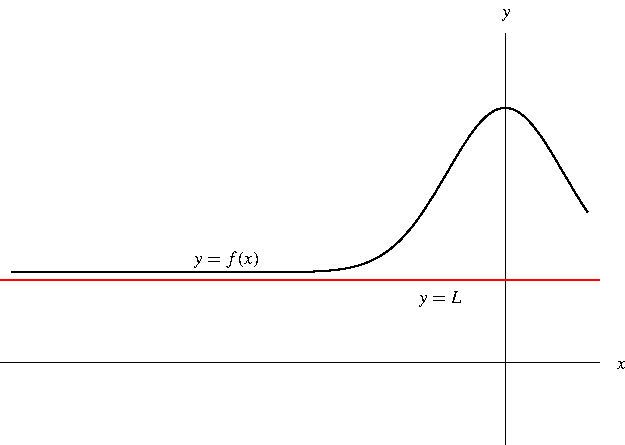
\includegraphics[width=6cm]{curve-sketching/pictures/04-04-negasymptotesa.pdf}%

\column{.5\textwidth}
\psset{xunit=0.7cm, yunit=0.7cm}
\begin{pspicture}(-5, -5)(5,5) 
\psframe*[linecolor=white](-7,-1)(1,3.5) 
\psaxes[ticks=none, labels=none]{<->}(0,0)(-6.5,-1)(1,3.5)
\rput[br](-3, 0.5){$y=f(x)$}
%Actual function formula: 1.5+2(4x)/(16x^2+1)
\psplot[linecolor=red, plotpoints=1000]{-7}{1}{1.5 x 8 mul 1 x 2 exp 16 mul add div add }
\psline[linestyle=dashed, linecolor=blue](-7, 1.5)(1,1.5)
\rput[br](-1, 1.6){$y=L$}
\end{pspicture}
%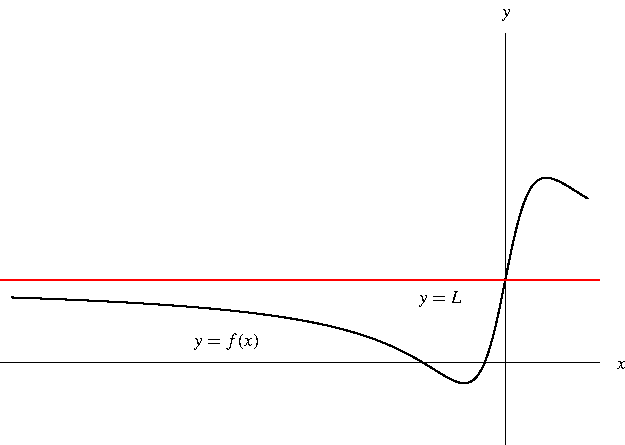
\includegraphics[width=6cm]{curve-sketching/pictures/04-04-negasymptotesb.pdf}%

\end{columns}
\end{frame}
% end module limit-at-infinity-def
